\documentclass[letterpaper,12pt]{article}
\usepackage{tabularx} % extra features for tabular environment
\usepackage{amsmath}  % improve math presentation
\usepackage{float}
\usepackage{pdfpages}


\usepackage{graphicx} % takes care of graphic including machinery
\graphicspath{ {./figures/} }
%\usepackage[margin=1in,letterpaper]{geometry} % decreases margins
%\usepackage{cite} % takes care of citations
\usepackage[final]{hyperref} % adds hyper links inside the generated pdf file
\hypersetup{
	colorlinks=true,       % false: boxed links; true: colored links
	linkcolor=blue,        % color of internal links
	citecolor=blue,        % color of links to bibliography
	filecolor=magenta,     % color of file links
	urlcolor =blue         
}
\usepackage[margin = 1in,headsep=0.5cm,headheight=2cm,letterpaper]{geometry} 

\usepackage{fancyhdr}
\pagestyle{fancy}
\lhead{Student 1 : Ahmet Akman 2442366 \\ Student 2: Yusuf Toprak Yıldıran 2444149 \\ Assistant: Onur Selim Kılıç}
\rhead{Date: \today \\ Group: Wednesday Morning - 5} 
%\cfoot{center of the footer!}
\renewcommand{\headrulewidth}{0.1pt}



\begin{document}
\thispagestyle{empty}

\title{Spring 2022 EE214 Experiment 3  \protect\\ Miscellaneous Op-Amp Circuits}
\author{Ahmet Akman 2442366 \protect\\ Yusuf Toprak Yıldıran 2444149 \protect\\ Assistant: Onur Selim Kılıç}
\date{\today}
\maketitle
\tableofcontents
%\begin{abstract}
%abstract
%\end{abstract}
\section{Introduction}

\section{Experimental Results and Discussion}
The results of the experiment are discussed in the following steps.
%
\subsection{Step 1}

In first step, following circuit given in Figure X is set and it is observed that step-down operation of the tansformer under no load with sinusoidal input voltage which has a peak to peak voltage of 20 V and frequency of 50 Hz. Then, \(V_{in}(t) \) and \(V_{out}(t)\) are plotted on the graph in Figure X.

Afterwards, \(N_1:N_2\) ratio is measured as \(\frac{19.5}{2.5}\approx 7.8 \).

%
\subsection{Step 2}
For this step, signal generator output is adjusted as \(V_s = 10sin(2\pi50t)\) with 20V peak to peak voltage and 50Hz frequency ;then, Transformer circuit with resistive load is constructed as given in the Figure X where R = \(56\Omega \).  
\subsubsection{i}
In this step, to obtain current \(I_{in}\), \(1K\Omega \) resistor is connected between - terminal of primary side transformer and - terminal of signal generator. Then, CH1 is connected to + terminal of the signal generator and CH2 probe is to the - terminal of primary side transformer. By subtracting CH2 from CH1 \(V_{in}\) is obtained, and CH2 probe of DSO gives \(I_{in}\) in mA. Afterwards, \(V_{in}\) and \(I_{in}\) are plotted in Figure X. Then, \(V_{rms}\) and \(I_{rms}\) are obtained using DSO measurement tool as 3.5V and 3.7mA respectively given in figure X. 
\begin{table}[H]
    \begin{center}
        \caption{RMS Values of input \(V_{rms}\) and input \(I_{rms}\)}
        \vspace{2mm}
        \begin{tabular}{||c | c ||} 
            \hline
            \(V_{rms}\) & \(I_{rms}\) \\ [0.5ex] 
            \hline\hline
            3.5 V & 3.7 mA    \\
            \hline
        \end{tabular}
    \end{center}
\end{table}

\subsubsection{ii}
For this step CH1 is connected to + terminal of secondary side of the transformer , and from that probe \(V_{out}(t)\) is obtained and plotted as in Figure X. Then, rms value of \(V_{out}\) is measured with DSO as 555mV.
\subsubsection{iii}
In this step, input frequency is increased to 500 Hz and i. and ii. are repeated. In previous steps (i. and ii.) phase difference between voltage and current was measured as \(-40\deg \) and when frequency is increased to 500 Hz phase difference is obtained as \(-25\deg\). Therefore, it is clearly seen that as frequency increase phase difference between voltage and current decreases. But after some point, although the frequency continues to increase, rate of change in phase difference decreases less and less.
%
\subsection{Step 3}

\subsubsection{i}
\subsubsection{ii}

%
\subsection{Step 4}
In this step impedance matching transformer circuit is constructed as if in Figure X with the input \(V_{in}(t) = 10sin(2\pi50t)\) and same \(N_1:N_2\) rate. 

\subsubsection{i}
For this step, impedance matching transformer circuit is used. In order to obtain \(V_{out}\) CH1 is connected + terminal of secondary side of the transformer and power dissipated on is calculated as follows:
\[\frac{V^2}{R} = \frac{(V_{rms})^2}{R} = \frac{0.216^2}{10\Omega } = 0.0046 Watt\]   

\subsubsection{ii}
For this step, 1K\(\Omega \) and 10\(\Omega \) resistors are connected series without the transformer and same calculation is made in i. :
\[\frac{V^2}{R} = 4.9 \times 10^{-4} Watt\]
 From these results, it is seen that in second case power transmitted to 10\(\Omega \) from the same input is significantly smaller than the first. Therefore, we can conclude that transformers can be used for delivering the power efficiently. 

\section{Conclusion}

\section*{Appendix A}
\begin{itemize}
    \item PreLab Preparation 4 hours
    \item Experimental Work 2  hours
    \item Report Writing 4 hours
\end{itemize}

\end{document}

%%%%%%%%%%%%%%%%%%%%%%   EXAMPLE TABLE   %%%%%%%%%%%%%%%%%%%%%%%%%%%%%%%%
\begin{table}[H]
\begin{center}
    \caption{Resistance reading by color code convention.}
    \vspace{2mm}
    \begin{tabular}{||c | c | c||} 
        \hline
        Color Order & Value & Tolerance \\ [0.5ex] 
        \hline\hline
        Brown / Black / Red / Gold & 1k\( \Omega \) & \( \% \) 5  \\ 
        \hline
        Yellow / Violet / Red / Gold & 4.7k\( \Omega \) & \( \% \) 5   \\
        \hline
        Brown / Grey / Orange / Gold & 18k\( \Omega \) & \( \% \) 5  \\ [1ex] 
        \hline
    \end{tabular}
\end{center}
\end{table}


%%%%%%%%%%%%%%%%%%%%%%   EXAMPLE IMAGE   %%%%%%%%%%%%%%%%%%%%%%%%%%%%%%%%
\begin{figure}[H]
\centering
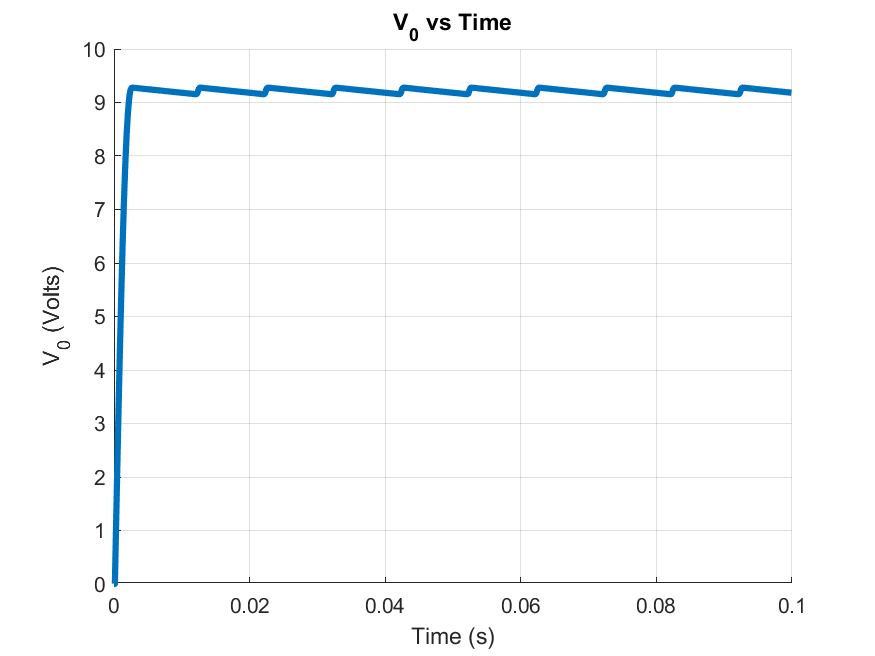
\includegraphics[width = 0.75\textwidth]{5.png}
\caption{Circuit schematic for the step 5}
\end{figure} 

%%%%%%%%%%%%%%%%%%%%%%   EXAMPLE IMAGE FROM PDF   %%%%%%%%%%%%%%%%%%%%%%%%%%%%%%%%
\begin{figure}[H] \centering{
	\includegraphics[scale=0.25]{2a_plot.pdf}}
	\caption{Experiment 2}
\end{figure}
	